\section{Introduction}
\label{sec:intro}

% Intro to Adaptive Analysis

The computational complexity of most problems is studied in the worst
case over instances of fixed size $n$, for $n$ asymptotically tending
to infinity. This approach was refined for NP-difficult problems under
the term ``parameterized
complexity''~\cite{2006-BOOK-ParameterizedComplexityTheory-FlumGrohe},
for polynomial problems under the term ``Adaptive
Algorithms''~\cite{1992-ACMCS-ASurveyOfAdaptiveSortingAlgorithms-EstivillCastroWood,1992-ACJ-AnOverviewOfAdaptiveSorting-MoffatPetersson},
and more simply for data encodings under the term of ``Data
Compression''~\cite{2013-TCS-OnCompressingPermutationsAndAdaptiveSorting-BarbayNavarro},
for a wide range of problems and data types.
Such a variety of results has motivated various tentative to classify
them, in the context of NP-hard problems with a theory of Fixed
Parameter
Tractability~\cite{2006-BOOK-ParameterizedComplexityTheory-FlumGrohe},
and in the context of sorting in the comparison model with a theory of
reduction between
parameters~\cite{1995-DAM-AFrameworkForAdaptiveSorting-PeterssonMoffat}.

% Examples of Results and Classification in Adaptive Analysis

In the context of ``Adaptive Analysis of Algorithms'', we introduce
two other perspectives from which to classify algorithms and data
structures: those taking advantage of the \emph{input order} (e.g.,
disorder measures for
\textsc{Sorting}~\cite{1992-ACJ-AnOverviewOfAdaptiveSorting-MoffatPetersson,1992-ACMCS-ASurveyOfAdaptiveSortingAlgorithms-EstivillCastroWood},
\textsc{Convex Hull}
algorithms~\cite{2002-SWAT-AdaptiveAlgorithmsForConstructingConvexHullsAndTriangulationsOfPolygonalChains-LevcopoulosLingasMitchell})
and those taking advantage of the \emph{input structure} (e.g., output
sensitive
algorithms~\cite{1986-JCom-TheUltimatePlanarConvexHullAlgorithm-KirkpatrickSeidel},
input order oblivious instance
optimality~\cite{2009-FOCS-InstanceOptimalGeometricAlgorithms-AfshaniBarbayChan}).

By \emph{input order} we mean algorithms taking advantage of the order
of the input, for example, taking advantage of the order of the values
in a sequence of numbers or of the order in which the points are given
in a polygonal chain.

Concerning the \textsc{Sorting} problem, as early as 1973,
Knuth~\cite{1973-BOOK-TheArtOfComputerProgrammingVol3-Knuth} described
a variant of the algorithm {\tt{MergeSort}} that sorts an array
$\mathcal{A}$ using a prepossessing step taking linear time to detect
maximal sorted subblocks, called \emph{runs}, in $\mathcal{A}$.
Takaoka~\cite{2009-Chapter-PartialSolutionAndEntropy-Takaoka}
described a new sorting algorithm that optimally takes advantage of
the distribution of the sizes of the runs in the array $\mathcal{A}$,
which yields a time complexity within
$O(n(1+\mathcal{H}(r_1, \dots, r_{\rho}))) \subseteq
O(n(1{+}\log{\rho})) \subseteq O(n\log{n})$, where $\rho$ is the
number of runs in $\mathcal{A}$ and $r_1, \dots, r_{\rho}$ are the
sizes of the $\rho$ \emph{runs} (such that $\sum_{i=1}^\rho {r_i}=n$),
respectively. Takaoka measures the ``difficulty'' of the instance in
terms of the ``input order'' by the entropy function
$\mathcal{H}(m_1, \dots, m_\sigma) =
\sum_{i=1}^\sigma{\frac{m_i}{n}}\log{\frac{n}{m_i}}$. These results
take advantage of the order of the values in the input i.e., the input
order.

Considering the computation of the {\sc{Convex Hull}} in the plane, Levcopoulos et al.~\cite{2002-SWAT-AdaptiveAlgorithmsForConstructingConvexHullsAndTriangulationsOfPolygonalChains-LevcopoulosLingasMitchell} described a divide-and-conquer algorithm for computing the {\sc{Convex Hull}} of a polygonal chain. The algorithm is based in the fact that the {\sc{Convex Hull}} of a simple chain can be computed in linear time, and that deciding whether a given chain is simple can be done in linear time.
They measured the complexity of this algorithm in terms of the minimum
number of simple subchains $\kappa$ into which the chain can be cut.
They showed that the time complexity of this algorithm is within
$O(n(1{+}\log{\kappa})) \subseteq O(n\log{n})$. This result takes advantage of the order in which the points are given i.e., the input order.

By ``input structure'' we mean algorithms taking advantage of the structure of the instance, for example, taking advantage of the frequencies of the values in a multiset or of the relative positions of the points in a set.

Concerning the {\sc{Sorting}} problem, Munro and
Spira~\cite{1976-JComp-SortingAndSearchingInMultisets-MunroSpira}
considered the task of {\sc{Sorting}} a multiset
$S=\{x_1, \dots, x_n\}$ of $n$ real numbers with $\sigma$ distinct
values, of multiplicities $m_1, \dots, m_\sigma$ (such that
$\sum_{i=1}^\sigma {m_i}=n$), respectively. They showed that adding
counters to various classical algorithms
\begin{INUTILE}
  (among which the divide-and-conquer based algorithm
  {\tt{MergeSort}})
\end{INUTILE}
yields a time complexity within
$O(n(1+\mathcal{H}(m_1, \dots, m_\sigma))) \subseteq
O(n(1{+}\log{\sigma})) \subseteq O(n\log{n})$ for {\sc{Sorting}} a
multiset. This result takes advantage of
the frequencies of the values i.e., the structure of the instance.

Considering the problem of computing the {\sc{Convex Hull}}, Kirkpatrick and Seidel~\cite{1986-JCom-TheUltimatePlanarConvexHullAlgorithm-KirkpatrickSeidel} described an algorithm to compute the {\sc{Convex Hull}} of a set of $n$ planar points in time within $O(n(1+\log h))\subseteq O(n\log n)$, where $h$ is the number of vertices in the {\sc{Convex Hull}}.
\begin{INUTILE}
  The algorithm relies on a variation of the divide-and-conquer
  paradigm, which they call the ``Marriage-Before-Conquest''
  principle.
\end{INUTILE}
Afshani et al.~\cite{2009-FOCS-InstanceOptimalGeometricAlgorithms-AfshaniBarbayChan} refined the complexity analysis of this algorithm to within $O(n(1+{\cal H}(n_1,\ldots,n_h)))\subseteq O(n(1{+}\log h)) \subseteq O(n\log{n})$, where $n_1, \dots, n_h$ are the sizes of a partition of the input, such that every element of the partition is a singleton or can be enclosed by a triangle whose interior is completely below the upper hull of the set, and ${\cal H}(n_1,\ldots,n_h)$ has the minimum possible value (minimum entropy of the distribution of the points into a certificate of the instance). This result takes advantage of the positions of the points i.e., the structure of the instance.

% Hypothesis

\paragraph{Hypothesis: Is it possible to combine both categories of
techniques into a single algorithm taking advantage of the input order
and the input structure in a synergistic way?}~\\

% Conclusion

Through the study of the sorting of multisets according to the
potential ``easiness'' in both the order and the values in the
multiset, in Section~\ref{sec:syn-sort} we show an
example of the difficulty of combining both into a single hybrid
algorithmic technique.
%
Through the study of the support of \texttt{rank} and
\texttt{select} queries on multisets according to the potential
``easiness'' in both the order and the values in the queries
themselves (in addition to the potential easiness in the data being
queried), in Section~\ref{sec:multiselect} and Section~\ref{sec:dds}
we extend the results to the context of \textsc{MultiSelection} and
\textsc{Deferred Data Structures}. These combinations yield a better
understanding of the problems and more efficient solutions which we
hope to extend to other problems (Section~\ref{sec:compressed},
Section~\ref{sec:maxima} and Section~\ref{sec:hull}).

\section{Sorting Solutions}
\label{sec:sort}

We review in Section~\ref{sec:back} the algorithms \texttt{MergeSort
  with Counters} described by Munro and
Spira~\cite{1976-JComp-SortingAndSearchingInMultisets-MunroSpira} and
\texttt{Minimal MergeSort} described by
Takaoka~\cite{2009-Chapter-PartialSolutionAndEntropy-Takaoka}, each
takes advantage of distinct features in the input. In Section
\ref{sec:syn-sort}, we describe two synergistic \textsc{Sorting}
algorithms, which never perform worse than \texttt{MergeSort with
  Counters} and \texttt{Minimal MergeSort}, and perform much better on
some large classes of instances by taking advantage of both the order
(local and global) and the structure in the input, in a synergistic
way. In Section~\ref{sec:multiselect}, we generalize one of the
algorithm described in Section~\ref{sec:syn-sort} to an offline
multiselection algorithm that partially sorts a multiset according to
the set of \texttt{select} queries given as input. In the context
where the queries arrive one at the time (i.e., online), in
Section~\ref{sec:dds} we define two \textsc{Deferred Data Structures}
for answering online \texttt{rank} and \texttt{select} queries, both
inspired by the \texttt{MultiSelection} algorithm.

\subsection{Background}
\label{sec:back}

The algorithm \texttt{MergeSort with Counters} described by Munro and
Spira~\cite{1976-JComp-SortingAndSearchingInMultisets-MunroSpira} is
an adaptation of the traditional sorting algorithm \texttt{MergeSort}
that optimally takes advantage of the structure in the input when
sorting a multiset $\mathcal{M}$ of size $n$. The algorithm divides
$\mathcal{M}$ into two equal size parts, sorts both parts recursively,
and then merges the two sorted lists. When two elements of same value $v$ are
found, one is thrown away and a counter holding the number of occurrences
of $v$ is updated. Munro and Spira measure the
``difficulty'' of the instance in terms of the ``input structure'' by
the entropy function
$\mathcal{H}(m_1, \dots, m_\sigma) =
\sum_{i=1}^\sigma{\frac{m_i}{n}}\log{\frac{n}{m_i}}$.  The time
complexity of the algorithm is within
$O(n(1 + \mathcal{H}(m_1, \dots, m_\sigma))) \subseteq
O(n(1{+}\log{\sigma})) \subseteq O(n\log{n})$, where $\sigma$ is the
number of distinct elements in $\mathcal{M}$ and
$m_1, \dots, m_\sigma$ are the multiplicities of the $\sigma$ distinct
elements in $\mathcal{M}$ (such that $\sum_{i=1}^\sigma {m_i}=n$),
respectively.

The algorithm \texttt{Minimal MergeSort} described by
Takaoka~\cite{2009-Chapter-PartialSolutionAndEntropy-Takaoka}
optimally takes advantage of the local order in the input, as measured
by the decomposition into runs when sorting an array $\mathcal{A}$ of
size $n$.  The main idea is to detect the runs first and then merge
them pairwise\begin{LONG}, using a \texttt{MergeSort}-like
  step\end{LONG}. The runs are detected in linear time\begin{LONG} by
  a scanning process identifying the positions $i$ in $\mathcal{A}$
  such that $\mathcal{A}[i] > \mathcal{A}[i+1]$\end{LONG}. Merging the
two shortest runs at each step further reduces the number of
comparisons, making the running time of the merging process adaptive
to the entropy of the sequence of the sizes of the runs.  The merging
process is then represented by a tree with the shape of a
Huffman~\cite{1952-IRE-AMethodForTheInstructionOfMinimumRedundancyCodes-Huffman}
tree, built from the distribution of the sizes of the \emph{runs}.  If
the array $\mathcal{A}$ is formed by $\rho$ runs and
$r_1, \dots, r_{\rho}$ are the sizes of the $\rho$ runs (such that
$\sum_{i=1}^\rho {r_i}=n$), then the algorithm sorts $\mathcal{A}$ in
time within
$O(n(1+\mathcal{H}(r_1, \dots, r_{\rho}))) \subseteq
O(n(1{+}\log{\rho})) \subseteq O(n\log{n})$.

The algorithm \texttt{MergeSort with Counters} is incomparable with
the algorithm \texttt{Minimal MergeSort}, in the sense that neither
one performs always better than the other. Simple modifications and
combinations of these algorithms do not take full advantage of both
the order (local and global) and structure in the input
(see~\cite{2016-ARXIV-SynergisticSortingAndDeferredDataStructuresOnMultiSets-BarbayOchoaSatty}
for detailed counter examples).

\subsection{Synergistic Sorting}
\label{sec:syn-sort}

In the following section we describe two sorting algorithms that take
the best advantage of both the order (local and global) and structure
in the input all at once when sorting a multiset. The first one is a
straightforward application of previous results, while the second one
prepares the ground for the \textsc{MultiSelection} algorithm
(Section~\ref{sec:multiselect}) and the \textsc{Deferred Data
  Structures} (Section~\ref{sec:dds}), which take
advantage of the order (local and global) and structure in the data
and of the order and structure in the queries.

\subsubsection{Sorting Algorithm \texttt{DLM
    Sort}}
\label{sec:dlm-sort}

In 2000, Demaine et
al.~\cite{2000-SODA-AdaptiveSetIntersectionsUnionsAndDifferences-DemaineLopezOrtizMunro}
described the algorithm \texttt{DLM Union}, an instance optimal algorithm that
computes the union of $\rho$ sorted sets.
\begin{LONG}
  It inserts the smallest element of each set in a heap. At each step,
  it deletes from the heap all the elements whose values are equal to
  the minimum value of the heap. If more than one element is deleted,
  it knows the multiplicity of this value in the union of the sets. It
  then adds to the heap the elements following the elements of minimum
  value of each set that contained the minimum value. If there is only
  one minimum element, it extracts from the heap the second minimum
  and executes a doubling
  search~\cite{1976-IPL-AnAlmostOptimalAlgorithmForUnboundedSearching-BentleyYao}
  in the set where the minimum belongs for the value of the second
  minimum. Once it finds the insertion rank $r$ of the second minimum
  (i.e., number of elements smaller than the second minimum in the set
  that contains the minimum), it also knows that the multiplicity of
  all elements whose positions are before $r$ in the set that contain
  the minimum are 1 in the union of the $\rho$ sets. These
    elements are discarded from future iterations of the
    algorithm. The process is repeated until all elements
  are discarded.
\end{LONG}\begin{SHORT}The algorithm scans the sets from left to right identifying blocks of
  consecutive elements in the sets that are also consecutive in the
  sorted union (see Figure~\ref{fig:instance} for a graphical
  representation of such a decomposition on a particular
  instance of the \textsc{Set Union} problem). In a minor way we refine their analysis as follow:
  
\end{SHORT}
\begin{LONG}
  
The time complexity of the \texttt{DLM Union} algorithm is measured in terms of the number and sizes of blocks of consecutive elements in the sets that are also consecutive in the sorted union (see Figure~\ref{fig:instance} where it is depicted an instance of the \textsc{Set Union} problem); the sizes of these blocks are referred to as \emph{gaps} in the analysis of the algorithm.\end{LONG} These blocks induce a partition $\pi$ of the output into intervals such that any singleton corresponds to a value that has multiplicity greater than $1$ in the input, and each other interval corresponds to a block as defined above. Each member $i$ of $\pi$ has a value $m_i$ associated with it: if the member $i$ of $\pi$ is a block, then $m_i$ is $1$, otherwise, if the member $i$ of $\pi$ is a singleton corresponding to a value of multiplicity $q$, then $m_i$ is $q$.
%
Let $\chi$ be the size of $\pi$.
%
If the instance is formed by $\delta$ blocks of sizes $g_1, \dots, g_{\delta}$ such that these blocks induce a partition $\pi$ whose members have values $m_1, \dots, m_{\chi}$, we express the time complexity of \texttt{DLM Union} as within $\Theta(\sum^{\delta}_{i=1}\log g_i + \sum^{\chi}_{i=1}\log{\binom{\rho}{m_i}})$.
%
This time complexity is within a constant factor of the complexity of any other algorithm computing the union of these sorted sets (i.e., the algorithm is instance optimal).

\begin{minipage}[c]{.45\textwidth}
  \centering
  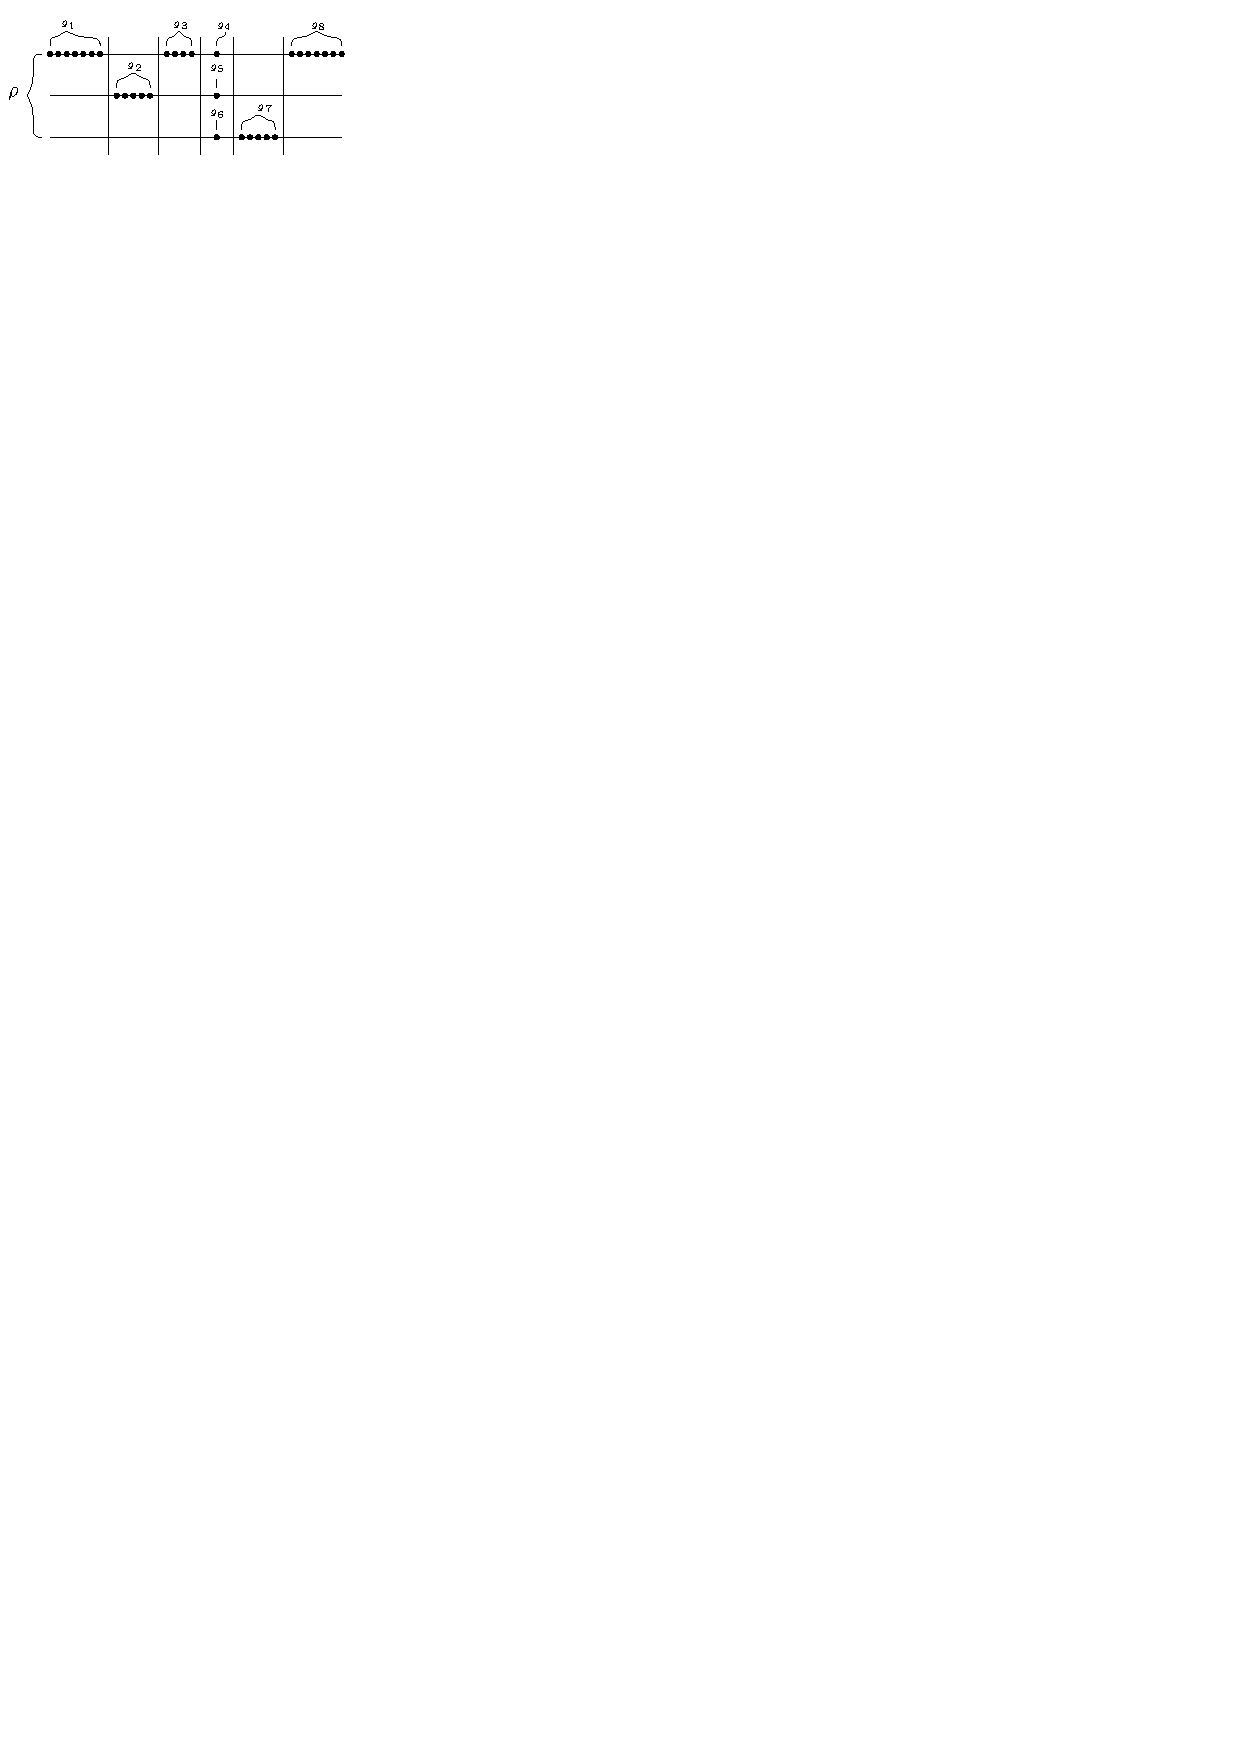
\includegraphics[scale=1.2]{union_instance1}
\end{minipage}\hfill
\begin{minipage}[c]{.45\textwidth}
  \captionof{figure}{An instance of the \textsc{Set Union} problem
    with $\rho=3$ sorted sets. In each set, the entry $\mathcal{A}[i]$ is
    represented by a point of $x$-coordinate $\mathcal{A}[i]$. The blocks
    that form the sets are noted. The blocks $g_4,g_5$ and $g_6$ are of
    size 1 because they correspond to elements of equal value and they
    induce the $4$-th member of the partition $\pi$ with value $m_4$
    equals $3$. The vertical bars separate the members of $\pi$.}
  \label{fig:instance}
\end{minipage}

We adapt the \texttt{DLM Union} algorithm for sorting a multiset.  The
algorithm \texttt{DLM Sort} detects the runs first through a linear
scan and then applies the algorithm \texttt{DLM Union}. After than,
transforming the output of the union algorithm to yield the sorted
multiset takes only linear time. The following corollary follows from
our refined analysis above:

\begin{corollary}
  Given a multiset $\mathcal{M}$ of size $n$ formed by $\rho$ runs and
  $\delta$ blocks of sizes $g_1, \dots, g_{\delta}$ such that these
  blocks induce a partition $\pi$ of size $\chi$ of the output whose
  members have values $m_1, \dots, m_{\chi}$, the algorithm {\tt{DLM Sort}} performs
  within
  $O(n + \sum^{\delta}_{i=1}\log g_i +
  \sum^{\chi}_{i=1}\log{\binom{\rho}{m_i}})$ data comparisons. This
  number of comparisons is optimal in the worst case over multisets of
  size $n$ formed by $\rho$ runs and $\delta$ blocks of sizes
  $g_1, \dots, g_{\delta}$ such that these blocks induce a partition
  $\pi$ of size $\chi$ of the output whose members have values
  $m_1, \dots, m_{\chi}$.
\end{corollary}

While the algorithm \texttt{DLM Sort} sorts multisets taking the best
advantage of both the \emph{input order} and the \emph{input
  structure} in a synergistic way, it does not yield a
\textsc{MultiSelection} algorithm nor a \textsc{Deferred Data
  Structure}. In the following section we
describe another sorting algorithm that also optimally takes advantage
of the local order and structure in the input, but which is based on a
distinct paradigm, more suitable to such extensions.

\subsubsection{Sorting Algorithm {\texttt{Quick Synergy
      Sort}}}
\label{sec:qss}

Given a multiset $\mathcal{M}$, the algorithm \texttt{Quick Synergy
  Sort} identifies the \emph{runs} in linear time through a scanning
process. \begin{LONG} As indicated by its name, the algorithm is
  directly inspired by the
  \texttt{QuickSort}~\cite{1961-CACM-Quicksort-Hoare}
  algorithm.\end{LONG} It computes a pivot $\mu$, which is the median
of the set formed by the middle elements of each run, and partitions
each \emph{run} by $\mu$. This partitioning process takes advantage of
the fact that the elements in each \emph{run} are already sorted. It
then recurses on the elements smaller than $\mu$ and on the elements
greater than $\mu$. (See Algorithm~\ref{alg:qss} for a more formal
description).

\begin{definition}[Median of the middles]
  Given a multiset $\mathcal{M}$ formed by runs, the ``\emph{median of
    the middles}'' is the median element of the set formed by the
  middle elements of each run.
\end{definition}

\begin{algorithm} % enter the algorithm environment
  \caption{\texttt{Quick Synergy Sort}} % give the algorithm a caption
  \label{alg:qss} % and a label for \ref{} commands later in the document
  \begin{algorithmic}[1] % enter the algorithmic environment

    \REQUIRE{A multiset $\mathcal{M}$ of size $n$} \ENSURE{A sorted sequence of
      $\mathcal{M}$}

    \STATE Compute the $\rho$ runs of respective sizes
    $(r_i)_{i\in[1..\rho]}$ in $\mathcal{M}$ such that
    $\sum^{\rho}_{i=1} r_i = n$;
    \STATE Compute the median $\mu$ of
    the middles of the runs, note $j\in[1..\rho]$ the run containing
    $\mu$;
    \STATE Perform doubling searches for the value $\mu$ in all
    runs except the $j$-th, starting at both ends of the runs in
    parallel;
    \STATE Find the maximum $\max_\ell$ (minimum $\min_r$)
    among the elements smaller (resp., greater) than $\mu$ in all runs
    except the $j$-th;
    \STATE Perform doubling searches for the values
    $\max_\ell$ and $\min_r$ in the $j$-th run, starting at the
    position of $\mu$;
    \STATE Recurse on the elements smaller than o
    equal to $\max_\ell$ and on the elements greater than or equal to
    $\min_r$.
  \end{algorithmic}
\end{algorithm}

The number of data comparisons performed by the algorithm
\texttt{Quick Synergy Sort} is asymptotically the same as the number
of data comparisons performed by the algorithm \texttt{DLM Sort}
described in the previous section.

\begin{theorem}
  Let $\mathcal{M}$ be a multiset of size $n$ formed by $\rho$ runs
  and $\delta$ blocks of sizes $g_1, \dots, g_{\delta}$ such that
  these blocks induce a partition $\pi$ of the output of size $\chi$
  whose members have values $m_1, \dots, m_{\chi}$. The algorithm
  \texttt{Quick Synergy Sort} performs within
  $O(n + \sum^{\delta}_{i=1} \log g_i +
  \sum^{\chi}_{i=1}\log{\binom{\rho}{m_i}})$ data comparisons on
  $\mathcal{M}$. This number of comparisons is optimal in the worst
  case over multisets of size $n$ formed by $\rho$ runs and $\delta$
  blocks of sizes $g_1, \dots, g_{\delta}$ such that these blocks
  induce a partition $\pi$ of size $\chi$ of the output whose members
  have values $m_1, \dots, m_{\chi}$.
\end{theorem}

\subsection{MultiSelection Algorithm}
\label{sec:multiselect}

\subsection{Deferred Data Structures for MultiSets}
\label{sec:dds}

\section{Compressed Data Structures}
\label{sec:compressed}

\section{Maxima Solutions}
\label{sec:maxima}

\section{Convex Hull Solutions}
\label{sec:hull}

We improve the analysis of this algorithm including not only the
minimum number of simple subchain into which the polygonal chain can
be partitioned but also their sizes.


\section{Conclusion}
\label{sec:con}

We predict that such analysis techniques will take on more importance
in the future, along with the growth of the block between practical
cases and the worst case over instances of fixed sizes. Furthermore,
we conjecture that synergistic techniques taking advantage of more
than one ``easiness'' aspect will be of practical importance if the
block between theoretical analysis and practice is to ever be reduced.

%%% Local Variables:
%%% mode: latex
%%% TeX-master: "2016-ThesisProposal-Ochoa"
%%% End:
